% Generated by Sphinx.
\def\sphinxdocclass{report}
\documentclass[a4paper,10pt,english]{sphinxmanual}
\usepackage[utf8]{inputenc}
\DeclareUnicodeCharacter{00A0}{\nobreakspace}
\usepackage[T1]{fontenc}
\usepackage{babel}
\usepackage{times}
\usepackage[Bjarne]{fncychap}
\usepackage{longtable}
\usepackage{sphinx}


\title{Qualimap Documentation}
\date{March 27, 2012}
\release{1.0}
\author{Fernando Garcia-Alcalde, et al}
\newcommand{\sphinxlogo}{}
\renewcommand{\releasename}{Release}
\makeindex

\makeatletter
\def\PYG@reset{\let\PYG@it=\relax \let\PYG@bf=\relax%
    \let\PYG@ul=\relax \let\PYG@tc=\relax%
    \let\PYG@bc=\relax \let\PYG@ff=\relax}
\def\PYG@tok#1{\csname PYG@tok@#1\endcsname}
\def\PYG@toks#1+{\ifx\relax#1\empty\else%
    \PYG@tok{#1}\expandafter\PYG@toks\fi}
\def\PYG@do#1{\PYG@bc{\PYG@tc{\PYG@ul{%
    \PYG@it{\PYG@bf{\PYG@ff{#1}}}}}}}
\def\PYG#1#2{\PYG@reset\PYG@toks#1+\relax+\PYG@do{#2}}

\def\PYG@tok@gd{\def\PYG@tc##1{\textcolor[rgb]{0.63,0.00,0.00}{##1}}}
\def\PYG@tok@gu{\let\PYG@bf=\textbf\def\PYG@tc##1{\textcolor[rgb]{0.50,0.00,0.50}{##1}}}
\def\PYG@tok@gt{\def\PYG@tc##1{\textcolor[rgb]{0.00,0.25,0.82}{##1}}}
\def\PYG@tok@gs{\let\PYG@bf=\textbf}
\def\PYG@tok@gr{\def\PYG@tc##1{\textcolor[rgb]{1.00,0.00,0.00}{##1}}}
\def\PYG@tok@cm{\let\PYG@it=\textit\def\PYG@tc##1{\textcolor[rgb]{0.25,0.50,0.56}{##1}}}
\def\PYG@tok@vg{\def\PYG@tc##1{\textcolor[rgb]{0.73,0.38,0.84}{##1}}}
\def\PYG@tok@m{\def\PYG@tc##1{\textcolor[rgb]{0.13,0.50,0.31}{##1}}}
\def\PYG@tok@mh{\def\PYG@tc##1{\textcolor[rgb]{0.13,0.50,0.31}{##1}}}
\def\PYG@tok@cs{\def\PYG@tc##1{\textcolor[rgb]{0.25,0.50,0.56}{##1}}\def\PYG@bc##1{\colorbox[rgb]{1.00,0.94,0.94}{##1}}}
\def\PYG@tok@ge{\let\PYG@it=\textit}
\def\PYG@tok@vc{\def\PYG@tc##1{\textcolor[rgb]{0.73,0.38,0.84}{##1}}}
\def\PYG@tok@il{\def\PYG@tc##1{\textcolor[rgb]{0.13,0.50,0.31}{##1}}}
\def\PYG@tok@go{\def\PYG@tc##1{\textcolor[rgb]{0.19,0.19,0.19}{##1}}}
\def\PYG@tok@cp{\def\PYG@tc##1{\textcolor[rgb]{0.00,0.44,0.13}{##1}}}
\def\PYG@tok@gi{\def\PYG@tc##1{\textcolor[rgb]{0.00,0.63,0.00}{##1}}}
\def\PYG@tok@gh{\let\PYG@bf=\textbf\def\PYG@tc##1{\textcolor[rgb]{0.00,0.00,0.50}{##1}}}
\def\PYG@tok@ni{\let\PYG@bf=\textbf\def\PYG@tc##1{\textcolor[rgb]{0.84,0.33,0.22}{##1}}}
\def\PYG@tok@nl{\let\PYG@bf=\textbf\def\PYG@tc##1{\textcolor[rgb]{0.00,0.13,0.44}{##1}}}
\def\PYG@tok@nn{\let\PYG@bf=\textbf\def\PYG@tc##1{\textcolor[rgb]{0.05,0.52,0.71}{##1}}}
\def\PYG@tok@no{\def\PYG@tc##1{\textcolor[rgb]{0.38,0.68,0.84}{##1}}}
\def\PYG@tok@na{\def\PYG@tc##1{\textcolor[rgb]{0.25,0.44,0.63}{##1}}}
\def\PYG@tok@nb{\def\PYG@tc##1{\textcolor[rgb]{0.00,0.44,0.13}{##1}}}
\def\PYG@tok@nc{\let\PYG@bf=\textbf\def\PYG@tc##1{\textcolor[rgb]{0.05,0.52,0.71}{##1}}}
\def\PYG@tok@nd{\let\PYG@bf=\textbf\def\PYG@tc##1{\textcolor[rgb]{0.33,0.33,0.33}{##1}}}
\def\PYG@tok@ne{\def\PYG@tc##1{\textcolor[rgb]{0.00,0.44,0.13}{##1}}}
\def\PYG@tok@nf{\def\PYG@tc##1{\textcolor[rgb]{0.02,0.16,0.49}{##1}}}
\def\PYG@tok@si{\let\PYG@it=\textit\def\PYG@tc##1{\textcolor[rgb]{0.44,0.63,0.82}{##1}}}
\def\PYG@tok@s2{\def\PYG@tc##1{\textcolor[rgb]{0.25,0.44,0.63}{##1}}}
\def\PYG@tok@vi{\def\PYG@tc##1{\textcolor[rgb]{0.73,0.38,0.84}{##1}}}
\def\PYG@tok@nt{\let\PYG@bf=\textbf\def\PYG@tc##1{\textcolor[rgb]{0.02,0.16,0.45}{##1}}}
\def\PYG@tok@nv{\def\PYG@tc##1{\textcolor[rgb]{0.73,0.38,0.84}{##1}}}
\def\PYG@tok@s1{\def\PYG@tc##1{\textcolor[rgb]{0.25,0.44,0.63}{##1}}}
\def\PYG@tok@gp{\let\PYG@bf=\textbf\def\PYG@tc##1{\textcolor[rgb]{0.78,0.36,0.04}{##1}}}
\def\PYG@tok@sh{\def\PYG@tc##1{\textcolor[rgb]{0.25,0.44,0.63}{##1}}}
\def\PYG@tok@ow{\let\PYG@bf=\textbf\def\PYG@tc##1{\textcolor[rgb]{0.00,0.44,0.13}{##1}}}
\def\PYG@tok@sx{\def\PYG@tc##1{\textcolor[rgb]{0.78,0.36,0.04}{##1}}}
\def\PYG@tok@bp{\def\PYG@tc##1{\textcolor[rgb]{0.00,0.44,0.13}{##1}}}
\def\PYG@tok@c1{\let\PYG@it=\textit\def\PYG@tc##1{\textcolor[rgb]{0.25,0.50,0.56}{##1}}}
\def\PYG@tok@kc{\let\PYG@bf=\textbf\def\PYG@tc##1{\textcolor[rgb]{0.00,0.44,0.13}{##1}}}
\def\PYG@tok@c{\let\PYG@it=\textit\def\PYG@tc##1{\textcolor[rgb]{0.25,0.50,0.56}{##1}}}
\def\PYG@tok@mf{\def\PYG@tc##1{\textcolor[rgb]{0.13,0.50,0.31}{##1}}}
\def\PYG@tok@err{\def\PYG@bc##1{\fcolorbox[rgb]{1.00,0.00,0.00}{1,1,1}{##1}}}
\def\PYG@tok@kd{\let\PYG@bf=\textbf\def\PYG@tc##1{\textcolor[rgb]{0.00,0.44,0.13}{##1}}}
\def\PYG@tok@ss{\def\PYG@tc##1{\textcolor[rgb]{0.32,0.47,0.09}{##1}}}
\def\PYG@tok@sr{\def\PYG@tc##1{\textcolor[rgb]{0.14,0.33,0.53}{##1}}}
\def\PYG@tok@mo{\def\PYG@tc##1{\textcolor[rgb]{0.13,0.50,0.31}{##1}}}
\def\PYG@tok@mi{\def\PYG@tc##1{\textcolor[rgb]{0.13,0.50,0.31}{##1}}}
\def\PYG@tok@kn{\let\PYG@bf=\textbf\def\PYG@tc##1{\textcolor[rgb]{0.00,0.44,0.13}{##1}}}
\def\PYG@tok@o{\def\PYG@tc##1{\textcolor[rgb]{0.40,0.40,0.40}{##1}}}
\def\PYG@tok@kr{\let\PYG@bf=\textbf\def\PYG@tc##1{\textcolor[rgb]{0.00,0.44,0.13}{##1}}}
\def\PYG@tok@s{\def\PYG@tc##1{\textcolor[rgb]{0.25,0.44,0.63}{##1}}}
\def\PYG@tok@kp{\def\PYG@tc##1{\textcolor[rgb]{0.00,0.44,0.13}{##1}}}
\def\PYG@tok@w{\def\PYG@tc##1{\textcolor[rgb]{0.73,0.73,0.73}{##1}}}
\def\PYG@tok@kt{\def\PYG@tc##1{\textcolor[rgb]{0.56,0.13,0.00}{##1}}}
\def\PYG@tok@sc{\def\PYG@tc##1{\textcolor[rgb]{0.25,0.44,0.63}{##1}}}
\def\PYG@tok@sb{\def\PYG@tc##1{\textcolor[rgb]{0.25,0.44,0.63}{##1}}}
\def\PYG@tok@k{\let\PYG@bf=\textbf\def\PYG@tc##1{\textcolor[rgb]{0.00,0.44,0.13}{##1}}}
\def\PYG@tok@se{\let\PYG@bf=\textbf\def\PYG@tc##1{\textcolor[rgb]{0.25,0.44,0.63}{##1}}}
\def\PYG@tok@sd{\let\PYG@it=\textit\def\PYG@tc##1{\textcolor[rgb]{0.25,0.44,0.63}{##1}}}

\def\PYGZbs{\char`\\}
\def\PYGZus{\char`\_}
\def\PYGZob{\char`\{}
\def\PYGZcb{\char`\}}
\def\PYGZca{\char`\^}
\def\PYGZsh{\char`\#}
\def\PYGZpc{\char`\%}
\def\PYGZdl{\char`\$}
\def\PYGZti{\char`\~}
% for compatibility with earlier versions
\def\PYGZat{@}
\def\PYGZlb{[}
\def\PYGZrb{]}
\makeatother

\begin{document}

\maketitle
\tableofcontents
\phantomsection\label{index::doc}



\chapter{Introduction}
\label{intro:introduction}\label{intro:intro}\label{intro::doc}

\section{What is Qualimap?}
\label{intro:what-is-qualimap}
Qualimap is a platform-independent application written in Java and R that provides both a Graphical User Interface (GUI) and a command-line interface to facilitate the quality control of alignment sequecing data. The aim of Qualimap is to provide an easy way for the quality control of mapping data, considering the sequence features and their genomic properties.

Basically, the application accepts and examines sequence alignment data, summarizing some interesting issues found in such data. The main features offered by Qualimap are: fast analysis across the reference genome of mapping coverage and nucleotide relative content; easy-to-interpret summary of the main properties of the alignment data; analysis of the reads mapped inside/outside of the regions defined in an annotation reference; analysis of the adequacy of the sequencing depth in RNA-seq experiments and clustering of !HERE!.


\section{Installation}
\label{intro:installation}
Download the ZIP archive with Qualimap from the \href{http://qualimap.org}{Qualimap web page}.

Unpack it to desired directory.

Now you can run Qualimap from this directory using the prebuilt script:

\samp{./qualimap}

Qualimap was tested on GNU Linux, MacOS and MS Windows. !Revise Windows!

\begin{notice}{note}{Note:}
On MS Windows use script qualimap.bat to launch Qualimap.
\end{notice}


\section{Requirements}
\label{intro:requirements}
Qualimap requires
\begin{itemize}
\item {} 
JAVA runtime (6 or above)

\item {} 
R enviroment (2.14 or above)

\end{itemize}

The JAVA runtime can be downloaded from the \href{http://www.java.com}{official web-site}.
There are prebuilt binaries available for many platforms.

R enviroment can be downloaded from \href{http://www.r-project.org}{R project web-site}.

Several Qualimap features are implemented in R, using a number of external packages.

\begin{notice}{note}{Note:}
If R enviroment is not availble, ``Epigenetics'' and ``RNA-seq'' features will be disabled.
\end{notice}

Currently Qualimap requires the following R-packages:
\begin{itemize}
\item {} 
optparse (available from \href{http://cran.r-project.org}{CRAN})

\item {} 
Repitools, Rsamtools, GenomicFeatures, rtracklayer (available from \href{http://bioconductor.org}{Bioconductor})

\end{itemize}

One can install these packages manually or use the script from Qualimap distribution.

Once R envronment is available the installation script can be invoked from Qualimap installation folder:

\samp{Rscript scripts/installDependencies.r}

\begin{notice}{note}{Note:}
In general the installation of R packages is platform-specific and may required additional effort.
\end{notice}


\section{Installing Qualimap on Ubuntu}
\label{intro:installing-qualimap-on-ubuntu}
This manual is specific for Ubuntu(Debian) Linux distributive !distributive?!, however with slight differences this can be applied for others Unix systems.


\subsection{Install JAVA}
\label{intro:install-java}
It is possible to use openjdk:

\samp{sudo apt-get install openjdk-6-jre}


\subsection{Install R}
\label{intro:install-r}
!Modify!
The R latest version can be installede from public repos.

However, the repos must be added to the sources. Open sources.list:

\samp{sudo gedit /etc/apt/sources.list}

Add the following lines:

\samp{deb http://\textless{}my.favorite.cran.mirror\textgreater{}/bin/linux/ubuntu \textless{}name.of.your.distribution\textgreater{}/}

Then install R:

\samp{sudo apt-get update}

\samp{sudo apt-get install r-base-core}

If you don't have the public key for the mirror add it:

\samp{gpg -{-}keyserver subkeys.pgp.net -{-}recv-key \textless{}required.key\textgreater{}}

\samp{gpg -a -{-}export \textless{}required.key\textgreater{} \textbar{} sudo apt-key add -}

More details available here:
\begin{quote}

\href{https://stat.ethz.ch/pipermail/r-help/2009-February/187644.html}{https://stat.ethz.ch/pipermail/r-help/2009-February/187644.html}

\href{http://cran.r-project.org/bin/linux/ubuntu/README}{http://cran.r-project.org/bin/linux/ubuntu/README}
\end{quote}

\begin{notice}{note}{Note:}
Alternatively it is possible to build R enviroment directly from sources downloaded from r-project.org.
\end{notice}


\subsection{Install required R-packages}
\label{intro:install-required-r-packages}
Use special script from Qualimap pacage:

\samp{Rscript \$QUALIMAP\_HOME/scripts/installDependencies.r}

where \samp{\$QUALIMAP\_HOME} is the full path to the Qualimap installation folder.


\chapter{Workflow}
\label{workflow:id1}\label{workflow::doc}\label{workflow:workflow}

\section{Starting a new analysis}
\label{workflow:starting-a-new-analysis}
To start new analysis activate main menu item \emph{File \(\rightarrow\) New Analysis} and select the desired type of analysis. Read more about different types of analysis {\hyperref[analysis:analysis-types]{\emph{here}}}.

{\hfill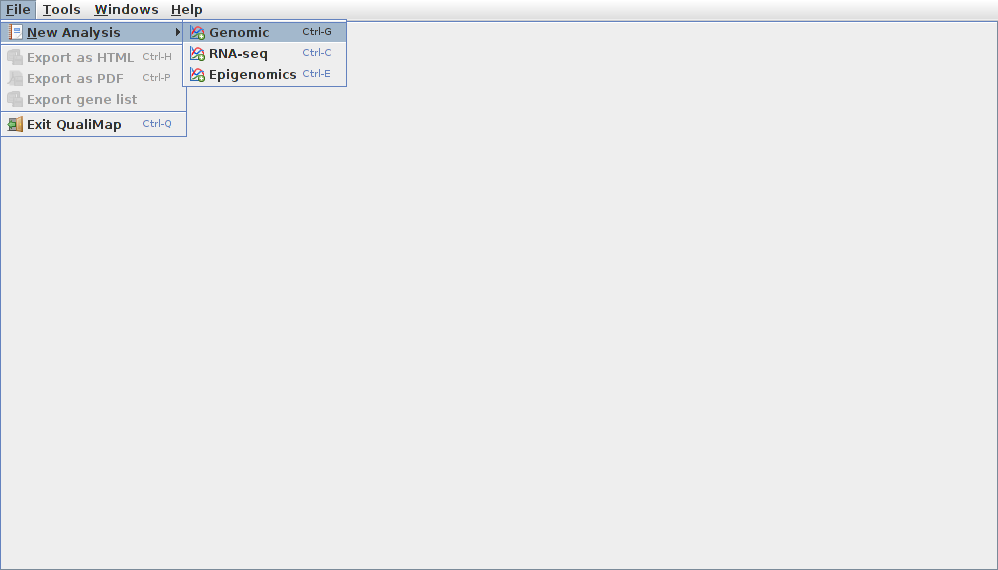
\includegraphics[width=500pt]{start_analysis3.png}\hfill}

After the corresponding item is selected a dialog will appear that allows customizing  analysis options (input  files, algorithm parameters, etc.).

{\hfill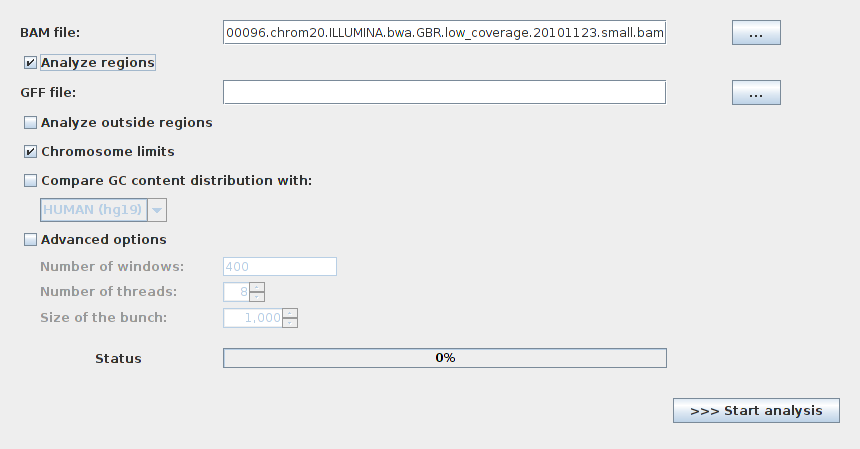
\includegraphics[width=500pt]{genomic3.png}\hfill}

To run the analysis click the \emph{Start analysis} button.

During the computation a status message and a graphic bar will indicate the progress of the computation.


\section{Viewing the results of the analysis}
\label{workflow:viewing-the-results-of-the-analysis}
After the selected analysis is finished the results are shown as an interactive report in the Qualimap main window. Several reports can be opened at the same time in different tabs.

In the left part of the report window one can find a list containing available result items. Clicking on an item will automatically show the corresponding information report or graph. Some report items are common for different types of analysis.

For example, \emph{Summary} section provides a short summary of performed quality control checks, while \emph{Input} section lists all the input parameters. Further information about each specific result is provided {\hyperref[analysis:analysis-types]{\emph{here}}}.


\section{Exporting results}
\label{workflow:exporting-results}
The resulting report can be saved to HTML page or PDF document.

To export results to HTML use a main menu item \emph{File \(\rightarrow\) Export to HTML}. In the appeared window one can select the path to the output folder. After clicking \emph{OK} button the web-page, containing analysis results will be saved to specified directory.

Similarly one can save the report to a PDF document by using a main menu item \emph{File \(\rightarrow\) Export to PDF}.


\section{Using tools}
\label{workflow:using-tools}
Qualimap provides also additional functionality other than quality control checks. The \emph{Tools} main menu item allows to access this functionality. Currently there is only one tool available -- {\hyperref[analysis:compute-counts]{\emph{Compute Counts}}}.

In future we plan to add more tools.


\chapter{Analysis types}
\label{analysis:analysis-types}\label{analysis::doc}\label{analysis:id1}

\section{Genomic}
\label{analysis:genomic}\label{analysis:id2}
Genomic analysis provides information for quality evaluation of the alignment data: base statistics summary showing mean GC-content, coverage, mapping quality and also a number of useful graphs, that allow to evaluate the quality of the sequencing data.


\subsection{Input}
\label{analysis:input}\begin{description}
\item[{\emph{BAM file}}] \leavevmode
Path to the sequence alignment file in BAM format. Note, that the BAM file has to be sorted. Sorting can be performed with \href{http://samtools.sourceforge.net/}{satmtools}.

\item[{\emph{Draw chromosome limits}}] \leavevmode
If selected, vertical dotted lines will be placed at the beginning of each chromosome according to the information found in the header of the BAM file.

\item[{\emph{Analyze regions}}] \leavevmode
Activating this option results in analysis of the alignment data only in specified region.

\item[{\emph{GFF file}}] \leavevmode
The path to the annotation file that specifies regions of interest.

\item[{\emph{Analyze outside regions}}] \leavevmode
This option allows to provide the information about the alignment data outside of the regions of interest. Useful for comparison purposes.

\item[{\emph{Compare GC content distribution with...}}] \leavevmode
Option allows to compare calculated distribution with selected precalculated genome distribution. Currently two genome distributions are available: human (hg19) and mouse (mm9)

\end{description}


\subsubsection{Advanced parameters}
\label{analysis:advanced-parameters}\begin{description}
\item[{\emph{Number of windows}}] \leavevmode
Number of windows used to split the selected genome reference. Default is 400.

\item[{\emph{Number of threads}}] \leavevmode
The genomic analysis computation can be performed in parallel on a multicore system using the given number of threads. The default number of threads equals number of available processors.

\item[{\emph{Reads per chunk}}] \leavevmode
To speed up the computation reads are analyzed in chunks. Each chunk is analyzed by single thread. This option controls the number of reads in a chunk. Smaller number may result in lower performance, but also the memory consumption will be reduced.

\end{description}


\subsection{Output}
\label{analysis:output}\begin{description}
\item[{\emph{Summary}}] \leavevmode
Basic information and statistics for the alignment sequencing input. For example, number of reads, number of mapped reads, mean coverage, chromosome-based statistics, etc.

\item[{\emph{Input data \& parameters}}] \leavevmode
Section provides the information about selected input parameters.

\item[{\emph{Coverage arcross reference}}] \leavevmode
This plot consists of two figures. The upper figure provides the coverage (red color) and coverage deviation across the reference sequence. The lower figure show gc-content across reference (black color) and it’s deviation.

\item[{\emph{Coverage}}] \leavevmode
Histogram Frequency histogram of the coverage.

\item[{\emph{Coverage histogram (0-50X)}}] \leavevmode
There is often big picks of coverage across the reference and the scale of the Coverage Histogram graph scale may not be adequate. In order to solve this, in this graph genome locations with a coverage greater than 50X are groped into the last bin.

\item[{\emph{Coverage quota}}] \leavevmode
Provides an easy way of viewing how much reference has been sequenced with a coverage higher than a selected level.

\item[{\emph{Mapped Reads Nucleotide Content}}] \leavevmode
This plot demonstrates the nucleotide content per read position.

\item[{\emph{Mapped Reads GC Content Distribution}}] \leavevmode
This graph shows the distribution of GC content per read. When compared with genome distribution this plot allows to check if there is a shift in the GC content.

\item[{\emph{Duplication Rate Histogram}}] \leavevmode
The histogram shows how many reads start at unique position. This plot is helpful to see if the fragment distribution across genome.

\item[{\emph{Mapping quality across reference}}] \leavevmode
Plot provides mapping quality across reference as indicate by the parameters.

\item[{\emph{Mapping quality histogram}}] \leavevmode
Histogram of the mapping quality frequency

\end{description}


\section{RNA-seq}
\label{analysis:rna-seq}\label{analysis:id3}
In RNA-seq experiments, the reads are mapped to a reference genome. If the total amount of sequencing reads is enough, the number of those reads mapping to a certain biological feature of interest (gene,
transcript, exon, ...) is an estimation of the abundance of that feature in the sample and can be used
as the quantification of its expression level.

These count data are usually utilized to assess differential expression between two or more experimental conditions. But before computing differential expression, users should be aware of some potential limitations of the RNA-seq data they are working with, as for example: has the saturation been reached or could more features be detected by increasing sequencing  depth? Which kind of features are being detected in the experiment? how good is the quantification of expression in the sample? All of these questions are easily answered by looking at the plots generated by Qualimap.

To study the quality of a sample from the count data in a RNA-seq experiment, please use the
RNA-seq option from the Analysis menu.

For this option to work, the R language must be installed in the user’s computer along with the R library “optparse” (both are freely available from \href{http://cran.r-project.org/}{http://cran.r-project.org/} ).


\subsection{Input}
\label{analysis:id4}\begin{description}
\item[{\emph{First sample (counts)}}] \leavevmode
File containing the count data from sample. Count data must be provided in a tab-delimited txt file, with the features names or IDs in the first column and counts in the second column. This file must not contain any header or column names. One can calculate the counts from a GFF file and a BAM file using option \emph{Tools \(\rightarrow\) Compute Counts}

\item[{\emph{First sample name}}] \leavevmode
Name for sample 1 to appear in plots legends

\item[{\emph{Second sample (counts)}}] \leavevmode
Optional. If a second sample is available, this file should contain the same information as in \emph{First sample}, but for the second sample. Mark the \emph{Compare with other sample} box to enable this option.

\item[{\emph{Second sample name}}] \leavevmode
Name for second sample to appear in plots legends.

\item[{\emph{Count threshold}}] \leavevmode
A feature is considered as detected if the corresponding number of counts isgreater than this count threshold. By default, the theshold value is set to 5 counts.

\item[{\emph{Info File}}] \leavevmode
Optional. File containing the biological classification of features in the count files. The info file must be a tab-delimited txt file, with the features names or IDs in the first column and the biological group (e.g. the biotype field from Biomart in the Ensembl database) in the second column. Again, the file must not contain any header or column names. If this file is provided, further exploratory plots can be generated to evaluate characteristics of the sample such us the kind of features being detected or the counts distribution for detected features. Please, make sure that the features IDs are the same in the \emph{Info file} and in the \emph{Count file}.

\item[{\emph{Species}}] \leavevmode
Optional. If the Info File is not given by the user, Qualimap provides the Ensembl biotype classification for certain species (human and  mouse in Qualimap version 1.0), whenever the features names in the counts file are the Ensembl gene or transcripts IDs (e.g. ENSG00000251282 or ENST00000508921). If so, mark the box to enable this option and select the species.

\end{description}


\subsection{Output}
\label{analysis:id5}
\emph{Global Saturation}
\begin{quote}

This plot provides information about the level of saturation in the sample, so it helps the user to decide if more sequencing is needed or if no many more features will detected when increasing the number of reads. These are some tips for the interpretation of the plot:
\begin{itemize}
\item {} 
The increasing sequencing depth of the sample is represented at the X-axis. The maximum value is the real sequencing depth of the sample(s). Smaller sequencing depths correspond to samples   randomly generated from the original sample(s).

\item {} 
The curve(s) is associated to the left Y-axis and represents the number of detected features when working with each of the sequencing depths in the X-axis. “Detected features” mean features with more than k counts, where k is the Count threshold chosen by the user.

\item {} 
The bars are associated to the right Y-axis and they represent the number of newly detected features when increasing the sequencing depth in one million reads at each sequencing depth value.

\end{itemize}
\end{quote}

When an \emph{Info File} is provided by the user or chosen from the ones supplied by Qualimap, a series of plots are additionally generated that are described next.
\begin{description}
\item[{\emph{Detection per group}}] \leavevmode
This barplot allows the user to know which kind of features are being detected in their sample(s). The X-axis shows all the biological groups included in the Info file (or the biotypes supplied by Qualimap). The grey bar is the percentage of features in each biological group within the reference genome (or transcriptome, etc.). The striped color bar is the percentage detected in the sample with regard to the genome. The solid color bar is the percentage that the group (or biotype) represents in the total detected features in the sample.

\item[{\emph{Counts per group}}] \leavevmode
A boxplot per each group (or biotype) describes the counts distribution for the detected features in that group.

\item[{\emph{Saturation per group}}] \leavevmode
For each group (or biotype), a saturation plot is generated like the one described above.

\item[{\emph{Counts \& Sequencing Depth}}] \leavevmode
For each group (or biotype), a plot is generated containing a boxplot with the distribution of counts at each sequencing depth. X-axis shows the increasing sequencing depths of randomly generated samples from the original one till the true sequencing depth is reached. This plot allows the user to see how the increase of sequencing depth is changing the expression level quantification.

\end{description}


\section{Epigenomic (Clustering)}
\label{analysis:epigenomic}\label{analysis:epigenomic-clustering}
This analysis type allows to cluster the regions of interest in the input alignment based on the coverage. Typical usecase for such clustering can be evaluation of epigenomics experiment. For example due to epigenetics changes When analyzing promoter regions one should expect some genes to be activated and some silenced.

To perform this evaluation you need to provide alignment data ( both methylated and control) and list of transcript ids as BED annotation file.


\subsection{Input}
\label{analysis:id6}\begin{description}
\item[{\emph{Experiment ID}}] \leavevmode
The experiment name

\item[{\emph{Alignment data}}] \leavevmode
Here you can provide your replicates to analyze. Each replicate includes sample file and a control file. For example, in an epigenomics experiment, the sample file could be the MeDIP-seq data and the control the non-encriched data (the so-called INPUT data). Thus, for each replicate the following information has to be provided:
\begin{description}
\item[{\emph{Replicate name}}] \leavevmode
Name of the replicate

\item[{\emph{Sample file}}] \leavevmode
Path to sample BAM file

\item[{\emph{Control file}}] \leavevmode
Path to control BAM file

\end{description}

To add a replicate click \emph{Add} button. To remove a replicate select it and click \emph{Remove} button. You can modify replicate by using \emph{Edit} button.

\item[{\emph{Regions of interest}}] \leavevmode
Path to an annotation file in BED format which contains regions of interest.
The BED file should be a tab delimited text file with exactly 6 fields per line:
\begin{itemize}
\item {} 
chromosome

\item {} 
start

\item {} 
end

\item {} 
name

\item {} 
score

\item {} 
strand (+ or -)

\end{itemize}

\item[{\emph{Location}}] \leavevmode
Relative location to analyze

\item[{\emph{Left offset}}] \leavevmode
Offset in bp upstream the selected regions

\item[{\emph{Right offset}}] \leavevmode
Offset in bp downstream the selected regions

\item[{\emph{Bin size}}] \leavevmode
Can be thought as the resolution of the plot. Bins of the desired size will be computed and the information falling on each bin will be aggregated

\item[{\emph{Number of clusters}}] \leavevmode
Number of groups that you the user wants to divide the data. Several values can be used by separting them with commas

\item[{\emph{Fragment length}}] \leavevmode
Length of the fragments that were initially sequenced. All reads will be enlarged to this length.

\item[{\emph{Visualization type}}] \leavevmode
You can visualize cluster using heatmaps or line-based graphs

\end{description}


\subsection{Output}
\label{analysis:id7}
After the analysis is performed, the regions of interest are clustered in groups based on the coverage pattern. The output graph shows the coverage pattern for each cluster either as a heatmap or a line graph. There can be multiple graphs based on the number of clusters provided as input. The name of each graph consists of the experiment name and the number of clusters.

It is possible to export list of features beloning to the particular cluster. To do this use main menu item \emph{File \(\rightarrow\) Export gene list} or context menu item \emph{Export gene list}. After activating the item a dialog will appear where you can choose some specific cluster. One can either copy the list of features belonging to this cluster in the clipboard or export it to a text file.


\section{Compute counts}
\label{analysis:id8}\label{analysis:compute-counts}
This tool allows to calculate how many reads belong to each region if interest in the alignment. To access the tool use menu item \emph{Tools \(\rightarrow\) Compute counts}.


\subsection{Input}
\label{analysis:id9}\begin{description}
\item[{\emph{BAM file}}] \leavevmode
Path to BAM alignment file

\item[{\emph{Annotation file}}] \leavevmode
Path to GTF file containing regions of interest

\item[{\emph{Protocol}}] \leavevmode
Three options are avalalbe:
\begin{description}
\item[{\emph{non-strand-specific}}] \leavevmode
Feature is counted independent of strand

\item[{\emph{forward-stranded}}] \leavevmode
Feature is counted only if it has the same strand as the read

\item[{\emph{reverse-strand}}] \leavevmode
Feature is counted only if the it has the strand reverse to the one of the read

\end{description}

\item[{\emph{Feature type}}] \leavevmode
Third column of the GTF file. Only features of this particular type are counted.

\item[{\emph{Feature name}}] \leavevmode
The name of the feature to be counted.

\item[{\emph{Output}}] \leavevmode
Path to the file which will contain output.

\item[{\emph{Save computation summary}}] \leavevmode
This option controls whether to save overall computation statistics.

\end{description}


\chapter{Command line interface}
\label{command_line:command-line-interface}\label{command_line::doc}\label{command_line:command-line}

\section{General description}
\label{command_line:general-description}
Each analysis type presented in QualiMap GUI is also available as command line tool. The common pattern to launch the tool is the following:

\begin{Verbatim}[commandchars=@\[\]]
qualimap @textless[]tool@_name@textgreater[] @textless[]tool@_options@textgreater[]
\end{Verbatim}

\emph{\textless{}tool\_name\textgreater{}} is the name of the desired analysis. This could be: {\hyperref[command_line:cmdline-genomic]{\emph{genomic}}}, {\hyperref[command_line:cmdline-rnaseq]{\emph{rna-seq}}}, {\hyperref[command_line:cmdline-epigenomic]{\emph{epigenomic}}} or {\hyperref[command_line:cmdline-counts]{\emph{counts}}}.

\emph{\textless{}tool\_options\textgreater{}} are specific to each type analysis. If not option is provided for the specific tool a full list of available options will be shown

To show available tools use command:

\begin{Verbatim}[commandchars=\\\{\}]
\PYG{n}{qualimap} \PYG{o}{-}\PYG{o}{-}\PYG{n}{help}
\end{Verbatim}


\section{Genomic}
\label{command_line:genomic}\label{command_line:cmdline-genomic}
The following command allows to perform genomic analysis:

\begin{Verbatim}[commandchars=@\[\]]
qualimap genomic -bam @textless[]arg@textgreater[] @PYGZlb[]-c@PYGZrb[] @PYGZlb[]-gff @textless[]arg@textgreater[]@PYGZrb[] @PYGZlb[]-home @textless[]arg@textgreater[]@PYGZrb[] @PYGZlb[]-nr @textless[]arg@textgreater[]@PYGZrb[] @PYGZlb[]-nt @textless[]arg@textgreater[]@PYGZrb[] @PYGZlb[]-nw @textless[]arg@textgreater[]@PYGZrb[] @PYGZlb[]-o@PYGZrb[] @PYGZlb[]-outdir @textless[]arg@textgreater[]@PYGZrb[] @PYGZlb[]-outformat @textless[]arg@textgreater[]@PYGZrb[]
-bam @textless[]arg@textgreater[]                     input mapping file
-c,--paint-chromosome-limits   paint chromosome limits inside charts
-gff @textless[]arg@textgreater[]                     region file (gff format)
-home @textless[]arg@textgreater[]                    home folder of Qualimap
-nr @textless[]arg@textgreater[]                      number of reads in the bunch (advanced)
-nt @textless[]arg@textgreater[]                      number of threads (advanced)
-nw @textless[]arg@textgreater[]                      number of windows (advanced)
-o,--outside-stats             compute region outside stats (only with -gff option)
-outdir @textless[]arg@textgreater[]                  output folder
-outformat @textless[]arg@textgreater[]               output report format (PDF or HTML, default is HTML)
\end{Verbatim}

\begin{DUlineblock}{0em}
\item[] 
\item[] The only required parameter is \emph{bam} -- the input mapping file.
\item[] If \emph{outdir} is not provided, it will be created automatically in the same folder where BAM file is located.
\item[] 
\item[] Detailed explanation of available options can be found {\hyperref[analysis:genomic]{\emph{here}}}.
\end{DUlineblock}

Example:

\begin{Verbatim}[commandchars=@\[\]]
./qualimap genomic -bam @textasciitilde[]/sample@_data/pl.bam -gff @textasciitilde[]/sample@_data/pl@_anns.gff --outside-stats
\end{Verbatim}


\section{RNA-seq}
\label{command_line:cmdline-rnaseq}\label{command_line:rna-seq}
To perform RNA-seq analysis use the following command:

\begin{Verbatim}[commandchars=@\[\]]
qualimap rna-seq -d1 @textless[]arg@textgreater[] @PYGZlb[]-d2 @textless[]arg@textgreater[]@PYGZrb[] @PYGZlb[]-home @textless[]arg@textgreater[]@PYGZrb[] @PYGZlb[]-i @textless[]arg@textgreater[]@PYGZrb[] @PYGZlb[]-k @textless[]arg@textgreater[]@PYGZrb[] @PYGZlb[]-n1 @textless[]arg@textgreater[]@PYGZrb[] @PYGZlb[]-n2 @textless[]arg@textgreater[]@PYGZrb[]
@PYGZlb[]-outdir @textless[]arg@textgreater[]@PYGZrb[] @PYGZlb[]-outformat @textless[]arg@textgreater[]@PYGZrb[] @PYGZlb[]-s @textless[]arg@textgreater[]@PYGZrb[]
-d1,--data1 @textless[]arg@textgreater[]      first file with counts
-d2,--data2 @textless[]arg@textgreater[]      second file with counts
-home @textless[]arg@textgreater[]            home folder of Qualimap
-i,--info @textless[]arg@textgreater[]        info file
-k,--threshold @textless[]arg@textgreater[]   threshold for the number of counts
-n1,--name1 @textless[]arg@textgreater[]      name for the first sample
-n2,--name2 @textless[]arg@textgreater[]      name for second sample
-outdir @textless[]arg@textgreater[]          output folder
-outformat @textless[]arg@textgreater[]       output report format (PDF or HTML, default is HTML)
-s,--species @textless[]arg@textgreater[]     use default file for the given species @PYGZlb[]human @textbar[] mouse@PYGZrb[]
\end{Verbatim}

\begin{DUlineblock}{0em}
\item[] 
\item[] Detailed explanation of available options can be found {\hyperref[analysis:rna-seq]{\emph{here}}}.
\end{DUlineblock}

Example:

\begin{Verbatim}[commandchars=@\[\]]
./qualimap rna-seq -d1 @textasciitilde[]/sample@_data/counts-kidney.txt -d2 @textasciitilde[]/sample@_data/counts-liver.txt -s human -outdir @textasciitilde[]/sample@_data/result
\end{Verbatim}


\section{Epigenomic}
\label{command_line:epigenomic}\label{command_line:cmdline-epigenomic}
To perform epigenomic analysis use the following command:

\begin{Verbatim}[commandchars=@\[\]]
qualimap epigenomic @PYGZlb[]-b @textless[]arg@textgreater[]@PYGZrb[] @PYGZlb[]-c @textless[]arg@textgreater[]@PYGZrb[] -control @textless[]arg@textgreater[] @PYGZlb[]-expr @textless[]arg@textgreater[]@PYGZrb[] @PYGZlb[]-f @textless[]arg@textgreater[]@PYGZrb[] @PYGZlb[]-home @textless[]arg@textgreater[]@PYGZrb[]
@PYGZlb[]-l @textless[]arg@textgreater[]@PYGZrb[] @PYGZlb[]-name @textless[]arg@textgreater[]@PYGZrb[] @PYGZlb[]-outdir @textless[]arg@textgreater[]@PYGZrb[] @PYGZlb[]-outformat @textless[]arg@textgreater[]@PYGZrb[] @PYGZlb[]-r @textless[]arg@textgreater[]@PYGZrb[] -regions @textless[]arg@textgreater[] -sample @textless[]arg@textgreater[] @PYGZlb[]-viz @textless[]arg@textgreater[]@PYGZrb[]
-b,--bin-size @textless[]arg@textgreater[]          size of the bin (default is 100)
-c,--clusters @textless[]arg@textgreater[]          comma-separated list of cluster sizes
-control @textless[]arg@textgreater[]               path to control BAM file
-expr @textless[]arg@textgreater[]                  name of the experiment
-f,--fragment-length @textless[]arg@textgreater[]   smoothing length of a fragment
-home @textless[]arg@textgreater[]                  home folder of Qualimap
-l @textless[]arg@textgreater[]                     left offset (default is 2000)
-name @textless[]arg@textgreater[]                  name of the replicate
-outdir @textless[]arg@textgreater[]                output folder
-outformat @textless[]arg@textgreater[]             output report format (PDF or HTML, default is HTML)
-r @textless[]arg@textgreater[]                     right offset (default is 500)
-regions @textless[]arg@textgreater[]               path to regions file
-sample @textless[]arg@textgreater[]                path to sample BAM file
-viz @textless[]arg@textgreater[]                   visualization type: heatmap or line
\end{Verbatim}

\begin{DUlineblock}{0em}
\item[] 
\item[] Detailed explanation of available options can be found {\hyperref[analysis:epigenomic]{\emph{here}}}.
\end{DUlineblock}

Example:

\begin{Verbatim}[commandchars=@\[\]]
./qualimap epigenomic -sample @textasciitilde[]/sample@_data/24h-i-medip.bam -control @textasciitilde[]/sample@_data/24h-i-control.bam -regions @textasciitilde[]/sample@_data/CpGislands.bed -outdir @textasciitilde[]/sample@_data/result
\end{Verbatim}


\section{Compute counts}
\label{command_line:cmdline-counts}\label{command_line:compute-counts}
To compute counts from mapping data use the following command:

\begin{Verbatim}[commandchars=@\[\]]
qualimap counts -bam @textless[]arg@textgreater[] @PYGZlb[]-f @textless[]arg@textgreater[]@PYGZrb[] -gff @textless[]arg@textgreater[] @PYGZlb[]-home @textless[]arg@textgreater[]@PYGZrb[] @PYGZlb[]-p @textless[]arg@textgreater[]@PYGZrb[]
-bam @textless[]arg@textgreater[]            mapping file in BAM format)
-f,--output @textless[]arg@textgreater[]     path to output file
-gff @textless[]arg@textgreater[]            region file in GFF format
-home @textless[]arg@textgreater[]           home folder of Qualimap
-p,--protocol @textless[]arg@textgreater[]   forward-stranded,reverse-stranded or non-strand-specific
\end{Verbatim}

\begin{DUlineblock}{0em}
\item[] 
\item[] Detailed explanation of available options can be found {\hyperref[analysis:compute-counts]{\emph{here}}}.
\end{DUlineblock}

Example:

\begin{Verbatim}[commandchars=@\[\]]
./qualimap counts -bam @textasciitilde[]/sample@_data/pl.bam -gff @textasciitilde[]/sample@_data/pl@_anns.bam
\end{Verbatim}



\renewcommand{\indexname}{Index}
\printindex
\end{document}
